\documentclass[acmlarge]{acmart}

\usepackage[
    type={CC},           % your choice
    modifier={by},       % your choice
    version={4.0},       % your choice
]{doclicense}            % your choice, see \doclicenseThis below

\settopmatter{printacmref=false}
\fancyfoot{}

\makeatletter
\def\@formatdoi#1{}
\def\@permissionCodeOne{miniKanren.org/workshop}
\def\@copyrightpermission{\doclicenseThis} % your choice of text
\def\@copyrightowner{Copyright held by the author(s).} % your choice
\makeatother

\copyrightyear{2019}
\setcopyright{rightsretained}

% Metadata Information
\acmJournal{PACMPL}
% \acmVolume{1}
% \acmNumber{ICFP} % CONF = POPL or ICFP or OOPSLA
\acmYear{2019}
\acmMonth{8}
\acmArticle{4}
% \acmDOI{} % \acmDOI{10.1145/nnnnnnn.nnnnnnn}

% \startPage{1}

\usepackage{booktabs} 
\usepackage{listings}
\usepackage[justification=centering]{caption}
\usepackage{subcaption}
% \usepackage{cite}
\usepackage{amssymb}
\usepackage{amsmath}
\usepackage{amsthm}
\usepackage{mathtools}
\usepackage{xspace}
\usepackage{bussproofs}
\usepackage{tikz}
\usepackage{float}
\usepackage{graphicx}
\usepackage{array}
\usepackage{tabularx}
\usepackage{collcell}
\usepackage[ruled]{algorithm2e} 

% \SetAlFnt{\small}
% \SetAlCapFnt{\small}
% \SetAlCapNameFnt{\small}
% \SetAlCapHSkip{0pt}
% \IncMargin{-\parindent}

% Paper history
% \received{February 2007}
% \received{March 2009}
% \received[accepted]{June 2009}

\bibliographystyle{ACM-Reference-Format}

\citestyle{acmauthoryear}

\newcommand{\rulehskip}{\hskip 1.5em}
\newcommand{\rulevspace}{\vspace{1em}}

\newcommand{\pvfill}{\pause\vfill}

% \mathchardef\mhyphen="2D

\theoremstyle{definition}

\newtheorem{example}{Example}[section]
\newtheorem{definition}{Definition}
\newtheorem{lemma}{Lemma}
\newtheorem{remark}{Remark}
\newtheorem{theorem}{Theorem}

\newenvironment{subproof}[1][\proofname]{%
  \renewcommand{\qedsymbol}{$\blacksquare$}%
  \begin{proof}[#1]%
}{%
  \end{proof}%
}

% \newtheorem{prop}{Proposition}

%% \counterwithin{lemma}{section}

\newcommand{\textdef}[1]{\textit{#1}}

\newcommand{\imm}{{\textrm IMM}~}

% inline code 
\newcommand{\code}[1]{\texttt{#1}}

% tuple with angle brackets
\newcommand{\tup}[1]{\langle #1 \rangle}

% semantics brackets
\newcommand{\sem}[1]{\llbracket #1 \rrbracket}

% equality by definition
\newcommand{\defeq}{\triangleq}

% function arrow
\newcommand{\fun}{\rightarrow}

% partial function arrow
\newcommand{\pfun}{\rightharpoonup}

% some math sets
\newcommand{\N}{{\mathbb{N}}}
\newcommand{\Q}{{\mathbb{Q}}}

% domain/codomain notation
\newcommand{\dom}[1]{\textit{dom}{({#1})}}
\newcommand{\codom}[1]{\textit{codom}{({#1})}}

\newcommand{\isground}[1]{\textit{is\_ground}({#1})}

\newcommand{\mgu}{\textit{mgu}}

\newcommand{\vars}[1]{\textit{Vars}({#1})}

\newcommand{\sapp}[2]{{#2}{#1}}
\newcommand{\subs}{\sqsubseteq}

% some logical notation
%\newcommand{\implies}{{\Rightarrow}}
%\newcommand{\iff}{{\Leftrightarrow}}

% check-mark and cross-mark
\newcommand{\cmark}{\text{\color{green!60!black}\ding{51}}}
\newcommand{\xmark}{\text{\color{red!60!black}\ding{55}}}

%% axiom labels

\newcounter{mylabelcounter}

\makeatletter
\newcommand{\labelAxiom}[2]{%
\hfill{\normalfont\textsc{(#1)}}\refstepcounter{mylabelcounter}
\immediate\write\@auxout{%
  \string\newlabel{#2}{{\unexpanded{\normalfont\textsc{#1}}}{\thepage}{{\unexpanded{\normalfont\textsc{#1}}}}{mylabelcounter.\number\value{mylabelcounter}}{}}
}%
}
\makeatother

%% warning

\colorlet{colorWARNING}{yellow!90!black}

% \newcommand{\warning}[1]{{\color{colorWARNING}\texttt{WARNING}}: #1}
% \newcommand{\app}[1]{{\color{blue}\textbf{ANTON: #1}}}
% \newcommand{\note}[1]{{\color{cyan}\textbf{EVG: #1}}}

\newcommand\ExecScaleFactor{1}

\newcommand{\todo}[1]{{\color{red}\textbf{TODO: #1}}}

%% OCanren's listings

\lstdefinelanguage{ocanren}{
    keywords={fresh, let, in, match, with, when, class, type,
    object, method, of, rec, repeat, until, while, not, do, done, as, val, inherit,
    new, module, sig, deriving, datatype, struct, if, then, else, open, private, virtual, include, success, failure,
    true, false},
    sensitive=true,
    commentstyle=\small\itshape\ttfamily,
    identifierstyle=\ttfamily,
    keywordstyle=\bfseries,
    basewidth={0.5em,0.5em},
    columns=fixed,
    fontadjust=true,
    abovecaptionskip=\bigskipamount,
    literate={->}{{$\to$}}3 {===}{{$\equiv$}}1 {=/=}{{$\not\equiv$}}1 {|>}{{$\triangleright$}}3  {/\\}{{$\wedge$}}2 {\\/}{{$\vee$}}2 {^}{{$\uparrow$}}1 {'}{{$^\prime$}}1 {~}{{$\neg$}}1 {=>}{{$\Rightarrow$}}2, 
    morecomment=[s]{(*}{*)}
}

\lstset{
    mathescape=true,
    %basicstyle=\small,
    commentstyle=\scriptsize\rmfamily,
    language=ocanren,
    captionpos=b,
    % escapeinside={(*}{*)},
}

\newcolumntype{H}{>{\collectcell\lstinline}l<{\endcollectcell}}

% Document starts
\begin{document}

% Title portion
\title{Constructive Negation for MiniKanren} 

\author{Evgenii Moiseenko}
%\authornote{with author2 note}          %% \authornote is optional;
                                        %% can be repeated if necessary
\orcid{nnnn-nnnn-nnnn-nnnn}             %% \orcid is optional
\affiliation{
  %\position{Position2a}
  %\department{}             %% \department is recommended
  \institution{Saint Petersburg State University}           %% \institution is required
  %\streetaddress{Street2a Address2a}
  \city{Saint Petersburg}
  %\state{Russia}
  %$postcode{Post-Code2a}
  %\country{Russia}                   %% \country is recommended
}
\email{e.moiseenko@2012.spbu.ru}         %% \email is recommended
\affiliation{
  %\position{Position2b}
  %\department{Department2b}             %% \department is recommended
  \institution{JetBrains Research}           %% \institution is required
  %\streetaddress{Street3b Address2b}
  %\city{City2b}
  %\state{State2b}
  %\postcode{Post-Code2b}
  %\country{Country2b}                   %% \country is recommended
  \country{Russia}
}
%\email{first2.last2@inst2b.org}         %% \email is recommended

\begin{abstract}

We present an extension of \textsc{MiniKanren} with the negation operator
based on the method of \emph{constructive negation}.
The idea of this method is to constructively 
build a stream of answers for the negated goal
by collecting and negating individual answers
to the positive version of the goal.
As we demonstrate on the series of examples 
constructive negation suits to pure logical nature of \textsc{MiniKanren}:  
the relations involving the negation operator 
still can be ``run'' in various directions.

\end{abstract}


%
% The code below should be generated by the tool at
% http://dl.acm.org/ccs.cfm
% Please copy and paste the code instead of the example below. 
%
\begin{CCSXML}
  <ccs2012>
    <concept>
      <concept_id>10011007.10011006.10011008.10011009.10011012</concept_id>
      <concept_desc>Software and its engineering~Functional languages</concept_desc>
      <concept_significance>500</concept_significance>
    </concept>
    <concept>
      <concept_id>10011007.10011006.10011008.10011009.10011015</concept_id>
      <concept_desc>Software and its engineering~Constraint and logic languages</concept_desc>
      <concept_significance>500</concept_significance>
    </concept>
  </ccs2012>
\end{CCSXML}

\ccsdesc[500]{Software and its engineering~Functional languages}
\ccsdesc[500]{Software and its engineering~Constraint and logic languages}

\keywords{relational programming, constructive negation, OCanren}

\maketitle
\thispagestyle{empty}

\section{Introduction}


  \begin{comment}
We implemented the synthesis framework using \textsc{OCanren}~--- an embedding of \textsc{miniKanren} into \textsc{OCaml}~\cite{ocanren},~---
 and evaluated it on the set of benchmarks, reported in the previous works on \emph{ad-hoc} algorithms for pattern matching
 code generation~\cite{maranget2001,maranget2008}. In comparison with a simplified setting, presented above, our implementation
 deals with a more elaborate pattern matching problem~--- in particular, we support \emph{guard expressions}, name bindings in
 patterns and incorporate a deterministic top-down matching strategy, which is common in functional languages.
 
 Initially, our synthesis did not demonstrate good results. However, we applied the following techniques to improve both the performance
 and the quality of synthesized programs:
 
 \begin{itemize}
 \item we restricted the shape of scrutinees using type information;
 \item we utilized tabling to memoize repeating search steps;
 \item we implemented a pruning technique, which makes the search stop exploring a certain branch if the program, synthesized so far,
   contains too much nesting constructs (this factor can be precomputed by patterns analysis).
 \end{itemize}
 
 With these adjustments, our synthesis framework in a negligible time provides the same results as those reported in the previous works.
 Our future steps include extending the pattern matching language to completely match that of \textsc{OCaml} (for
 now we do not support GADTs), integrate the synthesis into the existing \textsc{OCaml} compiler and evaluate it on a
 set of real-world programs. Another direction is extending the pattern matching language to incorporate features which
 are known to be hard, tedious or error-prone to implement (for example, non-linear patterns).
 
\end{comment}


\begin{comment}

Algebraic data types are essential for typed functional programming and it's difficult to imagine effective compiler without effective compilation of pattern matching. 
There are a few different approaches for compiling pattern mathcing. GHC is using influential paper~\cite{Jones1987}, OCaml is currently based on~\cite{maranget2001} although a work~\cite{maranget2008} can slightly improve effectiveness of generated code. 

Also there are a number of possible extensions of pattern matching itself (guards, non-linear patterns, active patterns) and extensions of possible matchable values (polymorphic variants in OCaml, for example). Although having all these extensions can be helpful for programming in practice, they can complicate compilation schema or make it very difficult to generate effective code. Supporting a large number  of extensions can seriously complicate compiler's implementation too.

We present an approach to pattern matching code generation based on application of relational programming~\cite{TRS,WillThesis} and, in
 particular, relational interpreters~\cite{unified}. We expect that our approach can compile pattern mathcing to competitive code and will be easier to support during adding of new pattern matching extensions.
 
\end{comment}
 We use a \emph{relational interpreter} for $\ir$
 
 \[
 eval^o_{\ir}\, (s, p, i)
 \]
 
 Here $s$ and $i$ have the same meaning as in declarative semantics description, $p\in\ir$~--- a syntactic representation of
 a program in $\ir$. The relation $eval^o_{\ir}$ encodes the operational semantics of $\ir$; it holds, if
 evaluating $p$ for $s$ returns $i$. Being relational interpreter, however, $eval^o_{\ir}$ is capable of solving a
 synthesis problem: by a scrutinee $s$ and a number $i$ calculate a program $p$ which makes the relation to hold.
 Within this setting, we can formulate the pattern-matching synthesis problem as follows: \emph{for a given ordered list of patterns $ps$ find a program $p$, such that}
 
 \[
 \forall s\in\mathcal{V},\,\exists i,\,eval^o_{\ir}\, (s, p, i) \wedge\, match (s, ps, i)
 \]
 
 It is rather problematic to directly solve this synthesis problem with existing \textsc{miniKanren} implementations as
 they provide a rather limited support for universal quantification~\cite{eigen,moiseenko}. However, in our concrete
 case there is a simple way to alleviate this problem. Indeed, we may replace universal quantification over $i$ by
 a finite conjunction, as the length of $ps$ is known at the synthesis time. As for the quantification over $s$, for
 any concrete $ps$ we may precompute a \emph{complete set of examples} $\mathcal{E}(ps)\subseteq\mathcal{V}$ with the following
 property:
 
 \[
 \forall i\in\mathbb{N},\,(\forall s\in\mathcal{E}(ps),\,match\, (s, ps, i) \Leftrightarrow \forall s\in\mathcal{V},\,match\, (s, ps, i))
 \]
 
 It easy to see, that for arbitrary $ps$ there exists a finite complete set of examples (indeed, any pattern describes the ``shape''
 of a scrutinee up to some finite depth, beyond which all scrutinees become indistinguishable). Thus, for a given $ps$ we may
 completely eliminate the quantification, reformulating the synthesis problem as
 
 \[
 \bigwedge_{i\in[1\dots|ps|]}\,\bigwedge_{s\in\mathcal{E}(ps)} (eval^o_{\ir}\, (s, p, i) \wedge match\, (s, ps, i))
 \]
 
 We implemented the synthesis framework using \textsc{OCanren}~--- an embedding of \textsc{miniKanren} into \textsc{OCaml}~\cite{ocanren},~---
 and evaluated it on the set of benchmarks, reported in the previous works on \emph{ad-hoc} algorithms for pattern matching
 code generation~\cite{maranget2001,maranget2008}. In comparison with a simplified setting, presented above, our implementation
 deals with a more elaborate pattern matching problem~--- in particular, we support \emph{guard expressions}, name bindings in
 patterns and incorporate a deterministic top-down matching strategy, which is common in functional languages.
 
 Initially, our synthesis did not demonstrate good results. However, we applied the following techniques to improve both the performance
 and the quality of synthesized programs:
 
 \begin{itemize}
 \item we restricted the shape of scrutinees using type information;
 \item we utilized tabling to memoize repeating search steps;
 \item we implemented a pruning technique, which makes the search stop exploring a certain branch if the program, synthesized so far,
   contains too much nesting constructs (this factor can be precomputed by patterns analysis).
 \end{itemize}
 
 With these adjustments, our synthesis framework in a negligible time provides the same results as those reported in the previous works.
 Our future steps include extending the pattern matching language to completely match that of \textsc{OCaml} (for
 now we do not support GADTs), integrate the synthesis into the existing \textsc{OCaml} compiler and evaluate it on a
 set of real-world programs. Another direction is extending the pattern matching language to incorporate features which
 are known to be hard, tedious or error-prone to implement (for example, non-linear patterns).
 
 \begin{comment}
 
 
 Real world modern compilers are obliged to address a few problems which are NP-complete and hence can't have effective
 algorithm to solve them. So, compilers use semi-optimal algorithms to find a decent solution. Optimal algorithms require
 brute force search to get the best solution and  affect compilation speed negatively. In this work we apply relational
 programming -- a convenient DSL for implementing search -- to compilation of pattern matching, one of a kind hard problems for compiler.
 
 The task of compiling pattern matching for typed languages is well presented in literature~\cite{maranget2001,maranget2008}.
 
 
 We test approach on simplified source language $PM$ where scrutinee is a value $\in\mathcal{V}$ of algebraic data type, only wildcards
 and nested constructors are allowed as patterns $\mathcal{P}$ and right hand side of clause is its index. The source language is easy
 extendable by pattern variables and optional pattern guards that test subterms of scrutinee using a function. The semantics of $PM$
 is a function from concrete scrutinee $s$, concrete patterns $pats$ and concrete guards $gs$ to clause indexes, and is denoted
 as $\sem{s,pats,gs}_{PM} = i$.
 
 Compilation scheme translates sentences from $PM$ to $\ir$ language which has constructions for clause indexes and conditions which
 test matchable values for specific constructor. Matchable values can be either a scrutinee, or a projection of matchable value that
 returns one of its field indexed by natural numbers. $\ir$ language is easy extendable by tests for fixed number of pattern guards.
 The semantics is straightforward and is denoted by $\sem{\cdot}_{\ir}$.
 
 We deal with a task of compiling pattern matching as it is a synthesis problem. The goal of algorithm is to synthesize $ideal_\ir$
 for concrete patterns $pats$ and guards that, firstly, will behave the same as original pattern matching for any possible
 scrutinee $s$. Secondly, we want shortest solution because short code usually runs faster. Relational programming~\cite{OCanren}
 will help with that because it has a tendency to generate short answers earlier, although this tendency is not strict.
 
 $$
 \forall s:\; \sem{s; ideal_\ir}_\ir = \sem{s;pats}_{PM}
 $$
 
 To eliminate universal quantifier we use the following observation: for \emph{finite} amount of patterns of \emph{finite} height
 we can generate \emph{finite} amount of examples to test pattern matching semantics. In examples, very deep subterms can have
 any value because they will not be tested during pattern matching. We can reformulate synthesis problem as follows:
 
 $$
 \mid  Examples\mid < \infty\quad \land\quad \left(\forall e \; (e\in Examples)\quad\land \quad\left( \sem{e; ideal_\ir}_\ir = \sem{e;pats}_{PM}\right)\right)
 $$
 
 For plain ADT the approach will generate required examples in finite time, but for GADTs it can diverge because inhabitancy problem
 is semi-decidable~\cite{garrigue2017gadts}(chapter 5). Inhabitants generation as well as synthesis algorithm is
 implemented\footnote{\url{https://github.com/Kakadu/pat-match/}} using relational programming.
 
 Presented approach is good as general description of an idea but require a few tweaks to start working, for example, on presented
 sample~\ref{fig:example1} . Firstly, synthesis procedure in a way as it is described doesn't take types into account, so it is
 useful to give hints about which parts of scrutinee should be checked for which constructors. Second observation says that we
 run $\sem{\cdot}_\ir$ in concrete direction, so it is possible to check periodically count of \texttt{IfTag} constructors in
 result value and prune branches where it becomes too big. Thirdly, synthesis query generates a lot of similar queries, and
 we use tabling to speedup search. All three observations are important, removing one of them leads to visible performance degradation.
 
 The optimal (two \texttt{IfTag}'s) and the semi-optimal solution (three \texttt{IfTag}'s) for~\ref{fig:example1} are described
 in~\cite{maranget2008}. Current implementation generates semi-optimal solution as 28th answer. Before that it generates optimal
 solution (and it's equivalents) three times, other 24 answers are longer and less useful. All tasks (example generation, synthesis
 and printing answers) take 3 seconds, which is unfortunate.
 
 Shortly, we present following contributions
 \begin{itemize}
 \item Code synthesis for pattern matching works after implementing \emph{three optimizations} above.
 \item GADTs, pattern binding and guards works for simple examples, the approach is easy extendable by them.
 \end{itemize}
 
 Future work is
 \begin{itemize}
 \item Discover other optimizations and enable current ones automatically using type information (at the moment we patched synthesis
   algorithm manually for concrete example).
 \item When current implementation tests for \texttt{cons} tag it can't propagate constraint that tag equals to \texttt{nil} to
   the \texttt{else} branch, which partially explains why branch pruning is so useful.
 \item Algorithm for inhabitant generation requires proper formulation and proof.
 \item Apply current synthesis procedure for exhaustiveness checking which will give us \emph{single} procedure for compilation and exhaustiveness checking.
 \item Test the approach on real world problems (embedding to OCaml compiler).
 \end{itemize}
 
 
 \begin{figure}[t]
   \[
   \begin{array}{rcll}
     \mathcal{C} & = & \{ C_1^{k_1}, \dots, C_n^{k_n} \}    &\mbox{(constructors)} \\
     \mathcal{V} & = & \mathcal{C}\,\mathcal{V}^*        &\mbox{(values)}       \\
     \mathcal{P} & = & \_ \mid \mathcal{C}\,\mathcal{P}^*&\mbox{(patterns)}     \\
     \mathcal{M} & = & \bullet \mid \mathcal{M} [\mathbb{N}]&
 
   \end{array}
   \]
 \end{figure}
 
 \begin{figure}
 \centering
 \begin{minipage}{.7\textwidth}
   \centering
 \begin{align*}
 \mathcal{C} =&\; \{ C_1^{k_1}, \dots, C_n^{k_n} \} \\
 \mathcal{V} =&\;  \mathcal{C}\ \mathcal{V}^*\\
 \mathcal{M} =&\;  \mathcal{S} \\
           \mid\; &\; \text{\texttt{Field}}\;  \mathcal{M}\times  \mathbb{N}\\
 \mathcal{P} =&\;  \text{\texttt{Wildcard}} \\
           \mid\; &\; \text{\texttt{Var}}\  Name\\
           \mid\; &\; \text{\texttt{PConstructor}}\  \mathcal{C}\times  \mathcal{P}^*\\
 \ir  =&\; \text{\texttt{Int}}\  \mathbb{N} \\
 %           \mid\; &\;\mathcal{S} \\
            \mid\; &\; \text{\texttt{IfTag}}\; \mathcal{C}\times \mathcal{M}\times \ir\times \ir\\
            \mid\; &\; \text{\texttt{IfGuard}}\ \mathbb{N}\times (Name\times \mathcal{M})^*\times \ir\times \ir\\
 Clause =&\;  \mathcal{P} \times \mathbb{N}? \times \ir
 \end{align*}
   \captionof{figure}{Structure of $PM$ and \ir languages}
 %  \label{fig:test1}
 \end{minipage}%
 \begin{minipage}{.3\textwidth}
   \centering
 \begin{lstlisting}[language=ocaml]
 match s with 
 | ([], _)     -> 1
 | (_, [])     -> 2
 | (_::_,_::_) -> 3
 \end{lstlisting}
   \captionof{figure}{Simple example of pattern matching problem from~\cite{maranget2008}}
 \label{fig:example1}
 \end{minipage}
 \end{figure}
 
 \end{comment}
 

\section{Examples}
\label{sec:examples}

In this section we present some examples of relational specification, written with the aid of our library.
Besides \miniKanren combinators themselves, our implementation contains two syntax extensions~--- one
for \lstinline{fresh} construct and another for \emph{inverse-$\eta$-delay}~\cite{MicroKanren}, which is
sometimes necessary to delay recursive calls in order to prevent infinite looping. In addition we included a
small relational library of data structures like lists, numbers, booleans, etc. This library is written
completely on the user level using techniques described in Section~\ref{sec:injection} with no utilization
of any unsafe features. The examples given below illustrate the usage of all these elements as well.

\subsection{List Concatenation and Reversing}

List concatenation and reversing are usually the first relational programs considered, and we do not wish
to deviate from this tradition. We've already considered the implementation of \lstinline{append$^o$} in
original \miniKanren in Section~\ref{sec:demo}. In our case, the implementation looks familiar:

\begin{lstlisting}
   let rec append$^o$ x y xy =
     (x === nil ()) &&& (y === xy) |||
     (fresh (h t)
       (x === h % t) &&&
       (fresh (ty)
         (h % ty === xy) &&& (append$^o$ t y ty)
       )
     )

   let rec revers$^o$ a b =
     conde [
       (a === nil ()) &&& (b === nil ());
       (fresh (h t)
         (a === h % t) &&&
         (fresh (a')
           (append$^o$ a' !< h b) &&& (revers$^o$ t a')
         )
       )
     ]
\end{lstlisting}

Here we make use of our implementation of relational lists, which provides convenient shortcuts for
standard functional primitives:

\begin{itemize}
  \item ``\lstinline{nil ()}'' corresponds to ``\lstinline{[]}'';
  \item ``\lstinline{h % t}'' corresponds to ``\lstinline{h::t}'';
  \item ``\lstinline{a %< (b %< (c !< d))}'' corresponds to ``\lstinline{[a; b; c; d]}''.
\end{itemize}

In our implementation the basic \miniKanren primitive ``\lstinline{conde}'' is implemented as a
disjunction of a list of goals, not as a built-in syntax construct. We also make use of explicit
conjunction and disjunction infix operators instead of nested bracketed structures which, we
believe, would look too foreign here.

\subsection{Relational Sorting and Permutations}

For the next example we take list sorting; specifically, we present a sorting for lists of natural numbers
in Peano form since our library already contains built-in support for them. However our example can be
easily extended for arbitrary (but linearly ordered) types.

List sorting can be implemented in \miniKanren in a variety of ways~--- virtually any existing algorithm can
be rewritten relationally. We, however, try to be as declarative as possible to demonstrate the
advantages of the relational approach. From this standpoint, we can claim that the sorted version of an empty list is an
empty list, and the sorted version of a non-empty list is its smallest element, concatenated with a sorted
version of the list containing all its remaining elements.

The following snippet literally implements this definition:

\begin{lstlisting}
   let rec sort$^o$ x y =
     conde [
       (x === nil ()) &&& (y === nil ());
       fresh (s xs xs')
         (y === s % xs')
         (sort$^o$ xs xs')
         (smallest$^o$ x s xs)
     ]
\end{lstlisting}

The meaning of the expression ``\lstinline{smallest$^o$ x s xs}'' is ``\lstinline{s} is the smallest element of a (non-empty) list \lstinline{x}, and \lstinline{xs} is the
list of all its remaining elements''. Now, \lstinline{smallest$^o$} can be implemented using a case analysis (note, ``\lstinline{l}'' here is a non-empty list):

\begin{lstlisting}
   let rec smallest$^o$ l s l' =
     conde [
       (l === s % nil ()) &&& (l' === nil ());
       fresh (h t s' t' max)
         (l' === max % t') &&&
         (l === h % t) &&&
         (minmax$^o$ h s' s max) &&&
         (smallest$^o$ t s' t')
     ]
\end{lstlisting}

Finally, we implement a relational minimum-maximum calculation
primitive:

\begin{lstlisting}
   let minmax$^o$ a b min max =
     conde [
       (min === a) &&& (max === b) &&& (le$^o$ a b);
       (max === a) &&& (min === b) &&& (gt$^o$ a b)
     ]
\end{lstlisting}

Here ``\lstinline{le$^o$}'' and ``\lstinline{gt$^o$}'' are built-in comparison goals for natural numbers in Peano form.

Having relational \lstinline{sort$^o$}, we can implement sorting for regular integer lists:

\begin{lstlisting}
   let sort l =
     run q (sort$^o$ @@ inj_nat_list l)
           (fun qs -> from_nat_list @@ (Stream.hd qs)#prj)
\end{lstlisting}

Here \lstinline{Stream.hd} is a function which takes a head from a lazy stream of answers,
\lstinline{inj_nat_list}~--- injection from regular integer lists into logical lists of logical Peano numbers,
\lstinline{from_nat_list}~--- projection from lists of Peano numbers to lists of integers.

It is interesting, that since \lstinline{sort$^o$} is
relational, it can be used to calculate the list of all \emph{permutations}
for a given list. Indeed, sorting each permutation results in the same list.
So, the problem of finding all permutations can be relationally reformulated into
the problem of finding all lists which are converted by sorting into the given one:

\begin{lstlisting}
let perm l = map (fun a -> a#prj |> from_nat_list) @@
  run q (fun q -> fresh (r)
                    (sort$^o$ (inj_nat_list l) r)
                    (sort$^o$ q r)
        )
        (Stream.take ~n:(fact @@ length l))
\end{lstlisting}

Note, for sorting the original list we used exactly the same primitive. Note also,
we requested exactly \lstinline{fact @@ length l} answers; requesting more
would result in an infinite search for non-existing answers.

\subsection{Type Inference for STLC}

Our final example is a type inferencer for Simply Typed Lambda Calculus~\cite{Lambda}. The problem and
solution themselves are rather textbook examples again~\cite{TRS, WillThesis}; however, with this example
we show once again the utilization of generic programming techniques we described in Section~\ref{sec:injection}.
As a supplementary generic programming library here we used object-oriented generic transformers\footnote{\url{https://github.com/dboulytchev/GT}};
we presume, however, that any other framework could equally be used.

We first describe the type of lambda terms and their logic representation:

\begin{lstlisting}
   module Term =
     struct
       module T =
         struct
           @type ('varname, 'self) t =
           | V   of 'varname
           | App of 'self    * 'self
           | Abs of 'varname * 'self
           with gmap

           let fmap f g x = gmap(t) f g x
         end

     include T
     include FMap2(T)

     let v   s   = inj @@ distrib @@ V s
     let app x y = inj @@ distrib @@ App (x, y)
     let abs x y = inj @@ distrib @@ Abs (x, y)
   end
\end{lstlisting}

Now we have to repeat the work for the type of simple types:

\begin{lstlisting}
   module Type =
     struct
       module T =
         struct
           @type ('a, 'b) t =
           | P   of 'a
           | Arr of 'b * 'b
           with gmap

          let fmap f g x = gmap(t) f g x
        end

       include T
       include FMap2(T)

       let p   s   = inj @@ distrib @@ P s
       let arr x y = inj @@ distrib @@ Arr (x, y)
     end
\end{lstlisting}

Note, the ``relational'' part is trivial, boilerplate and short (and could even be generated
using a more advanced framework).

The relational type inferencer itself rather resembles the original implementation. The only
difference (besides the syntax) is that instead of data constructors we use their logic
counterparts:

\begin{lstlisting}
   let rec lookup$^o$ a g t =
     fresh (a' t' tl)
       (g === (inj_pair a' t') % tl) &&&
       (conde [
         (a' === a) &&& (t' === t);
         (a' =/= a) &&& (lookup$^o$ a tl t)
       ])

   let infer$^o$ expr typ =
     let rec infer$^o$ gamma expr typ =
       conde [
         fresh (x)
           (expr === v x) &&&
           (lookupo x gamma typ);
         fresh (m n t)
           (expr === app m n) &&&
           (infer$^o$ gamma m (arr t typ)) &&&
           (infer$^o$ gamma n t);
         fresh (x l t t')
           (expr === abs x l) &&&
           (typ  === arr t t') &&&
           (infer$^o$ ((inj_pair x t) % gamma) l t')
       ]
     in
     infer$^o$ (nil()) expr typ
\end{lstlisting}

\section{Implementation}

\label{sec:implementation}

In this section we present our implementation of constructive negation.
We start with the general ideas behind the method (Section~\ref{sec:negation}).
We describe how the constructive negation behaves
in concrete examples, starting from trivial ones
and moving to more sophisticated.
During this presentation, we will observe, 
that in order to implement constructive negation, 
we need a solver for universally quantified disequality constraints.
We will show that such solver can be implemented 
on top of existing \textsc{MiniKanren} disequality solver
with just a few modifications (Section~\ref{sec:ctr-solver}).
In the Section~\ref{sec:search}, 
we describe how the \textsc{OCanren} search can be extended
to support constructive negation.
We will also discuss how negation interacts with recursion
and present the notion of \emph{stratification} (Section~\ref{sec:strat}). 

\subsection{General Ideas}

\label{sec:negation}

Constructive negation is based on the following idea: 
given a goal \lstinline{~g}, one can construct an answer for this goal 
by collecting all answers to its positive version \lstinline{g} 
and then taking their complementation.
In order to do that, a notion of ``negation'' of an answer is needed.
Since each answer can be matched to some logical formula~
\cite{przymusinski1989constructive, stuckey1991constructive}, 
a ``negation'' of an answer corresponds to the logical negation of
this formula. 

\begin{example}
  \label{ex:disequality}
  Consider the goal \lstinline{~(q === 1 /\ r === 2)}.
  Its positive version \lstinline{(q === 1) /\ (r === 2)} 
  has single answer, a substitution 
  $\mathtt{\{q \mapsto 1, r \mapsto 2 \}}$
  which corresponds to the formula $q = 1 \wedge r = 2$.
  By negating this formula we obtain $q \neq 1 \vee r \neq 2$.
  This formula still can be represent by a single substitution
  $\mathtt{\{q \mapsto 1, r \mapsto 2 \}}$.
  However, we now treat this substitution differently, as a \emph{disequality constraint}. 
\end{example}

Some \textsc{MiniKanren} implementations (including \textsc{OCanren})
already have the support for disequality constraints.
A programmer can use them with the help of 
\lstinline{=/=} primitive, as we have seen 
in the \lstinline{remove} example (Listing~\ref{lst:remove-correct}).
Usually, the support for disequalities is implemented as follows.

\begin{itemize}
  \item A current state is maintained during the search.
        The state consists of a substitution, 
        which represents positive information,
        and a disequality constraint store, 
        which represents negative information.
        A constraint store can be implemented simply 
        as a list of substitutions,
        or as a more efficient data structure.        

  \item Each time a subgoal of the form \lstinline{t =/= u} 
        is encountered during the search,
        its satisfiability in current substitution is checked.
        If it is satisfiable, then disequality 
        is added to the constraint store.

  \item Each time a subgoal of the form \lstinline{t === u} 
        is encountered during the search, 
        the current substitution is refined by the result 
        of unification of terms \lstinline{t} and \lstinline{u}. 
        Then the satisfiability of disequality constraints is rechecked 
        in the refined substitution.
\end{itemize}

Various optimizations can be applied to the scheme above.
For example, there is no need to recheck every 
disequality in the store after each unification.
We will not discuss these optimizations here, 
as they are irrelevant to our goals. 

Unfortunately, as the next example illustrates, 
disequalities presented above are not sufficient
to implement constructive negation.

\begin{example}
  \label{ex:univ-disequality}
  Consider a goal \lstinline{~(fresh (x) (q === (x, x))},
  which states that \lstinline{q} should not be equal to
  some pair of identical terms.
  The subgoal \lstinline{fresh (x) (q === (x, x))} succeeds,
  delivering the substitution $\mathtt{\{q \mapsto (x, x)\}}$.
  Because the variable \lstinline{x} occurs under \lstinline{fresh},
  the corresponding formula is existentially quantified:
  $\exists x\ldotp q = (x, x)$.
  By the negation of this formula we obtain 
  $\forall x\ldotp q \neq (x, x)$.
  This formula differs from disequality formula 
  from example~\ref{ex:disequality} as it 
  contains universally quantified variable \lstinline{x}.
\end{example}

Thereby, in order to support the negation of goals,
containing \lstinline{fresh},
we need to extend disequality constraint solver,
so it can check the satisfiability of 
\emph{universally quantified disequality constraints}
in the form $\forall \overline{x}\ldotp t \neq u$~\footnote{
$\overline{x}$ notation denotes a vector of variables,
$t$ and $u$ are terms that may or may not contain variables from $\overline{x}$
}~\cite{chan1988constructive, stuckey1991constructive}. 
Later, in Section~\ref{sec:ctr-solver} we will 
show how it can be done, for now let us assume we have such a solver. 

We took care about \lstinline{fresh} under negation.
It led us to a more complicated representation of the state. 
During the search we maintain a pair of a current substitution and 
a universally quantified disequality constraint store.
But now an interesting question arises: 
is this representation closed under negation? 
If we perform negation one more time, 
will we obtain a finite number of states in a similar form? 

Lucky for us, it is the case. In order to verify it, let us consider
a logical formula which corresponds to the representation of the state:

\begin{equation}
  \label{eq:state-positive}
  \exists\overline{x}\ldotp \left(
  \bigwedge_{i}(v_i = t_i) \wedge
  \bigwedge_{j}\forall\overline{y_j}\ldotp
  \bigvee_{k}(w_{jk} \neq u_{jk})
  \right)
\end{equation}

Here $v_i$ and $w_{jk}$ denote some variables,
$t_i$ and $u_{jk}$ denote some terms.
Existentially quantified variables $\overline{x}$
correspond to the variables occurred under \lstinline{fresh}.
The left conjunct corresponds to the substitution,
the right conjunct corresponds to the constraint store.
The constraint store itself is represented as a conjunction
of individual universally quantified disequalities.
As we have seen in example~\ref{ex:disequality},
each disequality corresponds to a disjunction
of individual inequalities over variables\footnote{
We will give further explanation in section~\ref{sec:ctr-solver}}.
Besides existential variables $\overline{x}$ 
and universal variables $\overline{y_j}$,
there are free variables $\overline{q}$ that may occur in the formula
(such as variables \lstinline{q} and \lstinline{r} in 
the examples~\ref{ex:disequality},~\ref{ex:univ-disequality}).

By logical negation of the above formula, we get the following:

\begin{equation}
  \label{eq:state-negation}  
  \forall\overline{x}\ldotp \left(
  \bigvee_{i}(v_i \neq t_i) \vee
  \bigvee_{j}\exists\overline{y_j}\ldotp
  \bigwedge_{k}(w_{jk} = u_{jk})
  \right)
\end{equation}

The left disjunct, which corresponded
to the substitution in the original formula, 
now became a disequality constraint. 
Looking at the right disjunct, 
we can see that each disequality 
has transformed into a substitution.
However, there is one subtlety here.
Variables $w_{jk}$ may be universally quantified,
that is $w_{jk} \in \overline{x}$ for some $j, k$.
Moreover, the terms $u_{jk}$ may contain universally quantified
variables as well, 
$\vars{u_{jk}} \subseteq \overline{x}$ for some $j, k$.
In the section~\ref{sec:ctr-solver} we will show,
that each disjunct  
$\exists\overline{y_j}\ldotp\bigwedge_{k}(w_{jk} = u_{jk})$ 
is either unsatisfiable or could be rewritten as 
$\exists\overline{y_j}\ldotp\bigwedge_{k^*}(w^*_{jk^*} = u^*_{jk^*})$,
such that universally quantified variables do not occur 
among variables $w^*_{jk^*}$ or in terms $u^*_{jk^*}$~\cite{liu1999constructive}. 

Taking this into account, we can rewrite the formula~\ref{eq:state-negation} as follow:

\begin{equation}
  \label{eq:state-negation-simpl}  
  (\bigvee_{j}\exists\overline{y_j}\ldotp
  \bigwedge_{k^*}(w^*_{jk^*} = u^*_{jk^*})) \vee
  \forall\overline{x}\ldotp
  \bigvee_{i}(v_i \neq t_i)
\end{equation}

In the obtained formula each disjunct corresponds to one state
in the form, similar to the given in formula~\ref{eq:state-positive}.
In the left disjunct, each sub-disjunct
corresponds to a substitution with an empty disequality constraint, 
the right disjunct corresponds to the 
single universally quantified disequality constraint 
with an empty substitution.
Thereby, the proposed representation of states
is closed under negation.

One can perform further manipulations on the formula~\ref{eq:state-negation-simpl}.
Given that equivalence $a \vee \neg b = a \wedge b \vee \neg b$ 
holds in classical logic, 
% and also 
% $\not\forall\overline{x}\ldotp\bigvee_{i}(u_i \neq t_i) = \exists\overline{x}\ldotp\bigwedge_{i}(u_i = t_i)$,
we can rewrite formula~\ref{eq:state-negation-simpl} in the following way:

\begin{equation}
  \label{eq:state-negation-rewritten}  
  (\exists\overline{x}\ldotp \bigwedge_{i}(v_i = t_i) \wedge 
   \bigvee_{j}\exists\overline{y_j}\ldotp
  \bigwedge_{k^*}(w^*_{jk^*} = u^*_{jk^*})) \vee
  \forall\overline{x}\ldotp
  \bigvee_{i}(v_i \neq t_i)
\end{equation}

The latter transformation,
while vacuous from the logical point of view,
could improve the performance of the search in practice.
It follows from the fact, that the subpart 
$\exists\overline{x}\ldotp \bigwedge_{i}(v_i = t_i)$ 
of the formula extends each substitution 
with additional mappings, 
thus delivering more positive information.
If the negation constitutes a subpart of some larger goal,
this positive information could lead to 
the earlier failure during the search.

Finally let us consider the negation in general case.
A goal can be matched to a logical formula in the following way.
Each answer to the goal corresponds to the state
which itself corresponds to a logical formula
in the form similar to one in formula~\ref{eq:state-positive}.
Goal can have multiple answers (even an infinite number).
In the corresponding logical formula these answers 
will be connected by the disjunction:

\begin{equation}
  \label{eq:positive-general}
  \bigvee_{n}\left(
  \exists\overline{x_{n}}\ldotp \left(
  \bigwedge_{i}(v_{ni} = t_{ni}) \wedge
  \bigwedge_{j}\forall\overline{y_{nj}}\ldotp
  \bigvee_{k}(w_{njk} \neq u_{njk})
  \right) \right)
\end{equation}

The negation of this formula after an application of the 
transformations described above will become:

\begin{equation}
  \label{eq:negation-general}  
  \bigwedge_{n}\left(
  (\exists\overline{x_{n}}\ldotp \bigwedge_{i}(v_{ni} = t_{ni}) \wedge 
   \bigvee_{j}\exists\overline{y_{nj}}\ldotp
  \bigwedge_{k^*}(w^*_{njk^*} = u^*_{njk^*})) \vee
  \forall\overline{x_n}\ldotp
  \bigvee_{i}(v_{ni} \neq t_{ni})
  \right)
\end{equation}

In this way, we have obtained the result of the negation of the goal
as a conjunction of the negation of individual answers to the 
positive version of the goal.
However, one of the pitfalls of this construction is 
that the process will not terminate if
the positive version of the goal has an infinite number of answers.
Thus, in the general case, it makes the \textsc{OCanren} search incomplete for the goals involving negation.

\subsection{Constraint Solver, Formally}

\label{sec:ctr-solver}

In this section we will formally define 
the satisfiability of universally quantified 
disequality constraints and quantified equalities,
mentioned in section~\ref{sec:negation}.
We will also present a simple decision procedure 
for satisfiability checking.
To do that we need a rather standard notions of  
terms, substitutions, unifiers, etc. 
For the sake of completeness we give these definitions here.
We also mention a standard unification algorithm as a
decision procedure for equality constraints.
This view of unification bridges the gap
between the conventional and constraint logic programming. 

Let us start with definitions of terms and substitutions.

\begin{definition}
  Given an infinite set of variables $V$ 
  and a finite set of constructor symbols $C = \{C^i_{n_i}\}_i$,
  each with associated arity $n_i$,
  the set of \emph{terms} $T$ is inductively defined as follow:
  \begin{itemize}
    \item $\forall v \in V \ldotp v \in T$ --- every variable is a term;
    \item $\forall c_k \in C\ldotp \forall t_1 \dots t_k \in T \ldotp c_k(t_1, \dots, t_k) \in T$ --- 
       every application of $k$-ary constructor symbol to $k$ terms is a term.
  \end{itemize}
\end{definition}

From now on we will assume that terms are untyped (unsorted)
and that there exists an infinitely many constructors of any arity.

\begin{definition}
  Two terms $t$ and $u$ are \emph{syntactically equal},
  denoted as $t = u$, iff either 
  \begin{itemize}
    \item $t = v$ and $s = v$ for some variable $v$;
    \item $t = c_k(t_1, \dots, t_k)$, $s = c_k(s_1, \dots, s_k)$ and
          $\forall i \in \{1 .. k\}\ldotp t_i = s_i$.
  \end{itemize}
\end{definition}

\begin{definition}
  A substitution $\sigma$ is a function 
  from variables to terms:
  $\sigma : V \fun T$,
  s.t. $\sigma(x) \neq x$ only for a finite number of variables.
  Every substitution $\sigma$ can be represented as 
  a finite list of pairs $\{x_1 \mapsto t_1, \dots, x_n \mapsto t_n \}$. 
  By $\dom{\sigma}$ we denote the set $\{x_1, \dots, x_n\}$
  and by $\codom{\sigma}$ we denote the set $\{t_1, \dots, t_n\}$.
  We denote empty substitution as $\top$.
  We also extend the set of substitutions defined above
  with the one additional element $\bot$.
\end{definition}

\begin{definition}
  A substitution can be \emph{applied to a term}.
  The result of an application of $\sigma$ ($\sigma \neq \bot$) to $t$,
  written as $\sapp{\sigma}{t}$, is a term defined 
  in the following way:
  \begin{itemize}
    \item $\sapp{\sigma}{x} \defeq \sigma(x)$;
    \item $\sapp{\sigma}{c_k(t_1, \dots, t_k)} \defeq c_k(\sapp{\sigma}{t_1}, \dots, \sapp{\sigma}{t_k})$.
  \end{itemize}
  The result of the application of $\bot$ to any term is undefined.
\end{definition}

\begin{lemma}
  \label{lemma:app}
  Given two substitutions $\sigma$ and $\theta$,
  if $\forall v \in V\ldotp \sigma(v) = \theta(v)$ 
  then $\forall t\ldotp \sapp{\sigma}{t} = \sapp{\theta}{u}$.
\end{lemma}

\begin{proof}
  Can be proved by the induction on $t$.
\end{proof}

We are now ready to define the  
the satisfiability of \emph{equality constraint}.

\begin{definition}
  \label{def:eq-ctr}
  Equality constraint $t \equiv u$ is 
  \begin{itemize}
    \item \emph{satisfiable} if $\exists \sigma\ldotp \sapp{\sigma}{t} = \sapp{\sigma}{u}$;
          such $\sigma$ is called a \emph{unifier} of $t$ and $u$;
    \item \emph{unsatisfiable} otherwise.
  \end{itemize}
\end{definition}

% \begin{remark}
%   \label{remark:ground-sat}
%   Strictly speaking, the definitions of satisfiability/unsatisfiability 
%   should involve ground terms. 
%   That is, proper definition of satisfiability of $t \equiv s$ should 
%   be given as follow:
%   \begin{itemize}
%     \item $t \equiv s$ \emph{satisfiable} if 
%           $\exists \sigma\ldotp \isground{\sigma} \wedge \sapp{\sigma}{t} = \sapp{\sigma}{s}$.
%   \end{itemize}
%   However, it is trivial to show, 
%   that in untyped case 
%   (assuming there is at least one 0-ary constructor symbol), 
%   if $t$ and $u$ are syntactically equal, 
%   then there exists a ground substitution $\sigma$,
%   such that $\sapp{\sigma}{t} = \sapp{\sigma}{s}$
%   Conversely, if $t$ and $u$ are not syntactically equal,
%   then there exists a ground substitution $\sigma$,
%   such that $\sapp{\sigma}{t} \neq \sapp{\sigma}{s}$
%   (with an additional assumption that there are at least two distinct constructor symbols).
%   Note that in the typed case it is not true.
%   For example, consider some variable $x$.
%   Clearly, $x$ is syntactically equal to itself, $x = x$.
%   Suppose that $x$ has type $\tau$.
%   If $\tau$ is uninhabited then there is no ground terms of type $\tau$,
%   and thus there is no ground substitution for $x$.
% \end{remark}

Next, we show that the standard unification algorithm
can be seen as a decision procedure 
for checking satisfiability of equality constrains.
Before that we need to introduce several definitions.

\begin{definition}
  A term $t$ is \emph{subsumed} by the term $u$, 
  denoted as $t \subs u$,
  iff $\exists \sigma\ldotp t = \sapp{\sigma}{u}$.
  If $t \subs u$ we will also say that 
  $t$ \emph{is a more specific} term than $u$,
  or $u$ \emph{is a more general} term than $t$.
\end{definition}

\begin{definition}
  A substitution $\sigma$ is \emph{subsumed} by a substitution $\tau$, 
  denoted as $\sigma \subs \tau$,
  iff $\forall t\ldotp \sapp{\sigma}{t} \subs \sapp{\tau}{t}$.
  If $\sigma \subs \tau$ we also say that 
  $\sigma$ \emph{is a more specific substitution} than $\tau$,
  or $\sigma$ \emph{is a more general substitution} than $\tau$.
\end{definition}

\begin{definition}
  \label{def:mgu}
  Given terms $t$ and $u$ their unifier $\sigma$ is called the
  \emph{most general unifier}, 
  iff for every other unifier $\tau$
  $\sigma$ is more general that $\tau$, $\tau \subs \sigma$.
\end{definition}

\begin{theorem}
  \label{lemma:unify}
  Given terms $t$ and $u$ they are either not unifiable 
  (meaning that $\forall \sigma\ldotp \sapp{\sigma}{t} \neq \sapp{\sigma}{u}$),
  or there exists their most general unifier.
\end{theorem}

\begin{proof}
  Proof of this statement can be found in~\cite{robinson1965machine}.
  Proof of the termination and correctness of the unification algorithm,
  used by the most \textsc{MiniKanren} implementations,
  can be found in~\cite{kumar2010nominal}.
\end{proof}

From now on we will denote the most general unifier
of two terms $t$ and $u$ as $\mgu(t, u)$.
In case of $t$ is not unifiable with $u$,
we assume that $\mgu(t, u) = \bot$.

\begin{remark}
  Note we can associate with an 
  equality constraint $t \equiv u$ a
  logical first-order formula $t = u$.
  % Then, given the remark~\ref{remark:ground-sat}, 
  % the satisfiability of the constraint $t \equiv u$
  % implies the satisfiability of the formula.
  Additionally, we can associate with each substitution a logical first-order formula
  by the following rules:
  \begin{itemize}
    \item empty substitution $\top$ is associated with the truth constant $\top$;
    \item $\bot$ is associated with the falsity constant $\bot$;
    \item $\{x_1 \mapsto t_1, \dots, x_n \mapsto t_n\}$ is associated with 
          the formula $x_1 = t_1 \wedge \dots \wedge x_n = t_n$.
  \end{itemize}
  Now we can have yet another view on unification.
  We can say that giving the problem of deciding satisfiability
  of the formula $t = u$, a unification algorithm reduces it 
  to checking satisfiability of a simpler formula,
  which corresponds to a substitution. 
  Such a formula is either trivially unsatisfiable 
  (in the case of $\bot$) or trivially satisfiable.
\end{remark}

% \begin{example}
%   \label{ex:equality-sat}
%   \todo{example of unification/equality constraint}
% \end{example}

Later on we will need the notion of idempotent substitution and idempotent unifier.

\begin{definition}
  \label{def:idempotent-subs}
  Substitution $\sigma$ is \emph{idempotent} iff
  $\forall t\ldotp \sapp{\sigma}{\sapp{\sigma}{t}} = \sapp{\sigma}{t}$
\end{definition}

\begin{lemma}
  \label{lemma:idempotent-unif}
  If two terms are unifiable, there exists their idempotent unifier.
\end{lemma}

\begin{proof}
  For the proof of this statement 
  (for the case of unification algorithm, used in \textsc{MiniKanren}),
  we refer an interested reader to~\cite{kumar2010nominal}.
\end{proof}

We are ready to move on to disequality constraints.
We start with the regular (not quantified) disequalities.

\begin{definition}
  \label{def:diseq-sat}
  A disequality constraint $t \not\equiv u$ is 
  \begin{itemize}
    \item \emph{satisfiable} if $\exists \sigma\ldotp \sapp{\sigma}{t} \neq \sapp{\sigma}{u}$;
    \item \emph{unsatisfiable} otherwise.
  \end{itemize}
\end{definition}

Next lemma gives us a simple decision procedure for checking 
satisfiability of disequalities.

\begin{lemma}
  \label{lemma:diseq-sat}
  Disequality constraint $t \not\equiv u$ is 
  \begin{itemize}
    \item \emph{satisfiable} if $\mgu(t, u) \neq \top$;
    \item \emph{unsatisfiable} otherwise.
  \end{itemize}
\end{lemma}

\begin{proof}
  Let $\theta = \mgu(t, u)$.
  Let us first show that if $\theta = \top$ 
  then disequality is unsatisfiable.
  By the definition of $\top$ we have 
  $\sapp{\theta}{t} = t$ and $\sapp{\theta}{u} = u$,
  by the definition of unifier 
  $\sapp{\theta}{t} = \sapp{\theta}{u}$, 
  and thus $t = u$.
  From that, it is easy to show that 
  $\forall \sigma\ldotp \sapp{\sigma}{t} = \sapp{\sigma}{s}$,
  which means that the disequality is unsatisfiable according to 
  the definition~\ref{def:diseq-sat}.
  If $\theta \neq \top$ then 
  there exists a substitution $\sigma$,
  s.t. $\theta \subs \sigma$ (e.g. $\sigma = \top$).
  Since $\theta$ is most general unifier, 
  and $\sigma$ is more general that $\theta$,
  then $\sigma$ is not a unifier,
  and thus $\sapp{\sigma}{t} \neq \sapp{\sigma}{u}$.
\end{proof}

Given lemma~\ref{lemma:diseq-sat}, the satisfiability of
constraint $t \not\equiv u$ can be checked easily.
One need to compute $\mgu(t, u)$
and if it is not an empty substitution,
then constraint is satisfiable.

\begin{remark}
  Given disequality constraint $t \not\equiv u$,
  a substitution $\mgu(t, u)$,
  can be matched to the logical formula in the following way:
  \begin{itemize}
    \item the empty substitution $\top$ is associated with falsity constant $\bot$;
    \item $\bot$ is associated with the truth constant $\top$;
    \item $\{x_1 \mapsto t_1, \dots, x_n \mapsto t_n\}$ is associated with 
          the formula $x_1 \neq t_1 \vee \dots \vee x_n \neq t_n$.
  \end{itemize}
\end{remark}

% \begin{example}
%   \label{ex:disequality-sat}
%   \todo{example of disequality constraint}
% \end{example}

The following definition introduces universally quantified disequalities.

\begin{definition}
  Universally quantified disequality constraint 
  $\forall \overline{x}\ldotp t \not\equiv u$ is
  \begin{itemize}
    \item \emph{satisfiable} iff
          ${\exists \sigma\ldotp 
            \forall \tau, \dom{\tau} \subseteq \overline{x}\ldotp 
            \sapp{\sigma}{\sapp{\tau}{t}} \neq \sapp{\sigma}{\sapp{\tau}{u}}
          }$
    \item \emph{unsatisfiable} iff
          ${\forall \sigma\ldotp 
            \exists \tau, \dom{\tau} \subseteq \overline{x}\ldotp 
            \sapp{\sigma}{\sapp{\tau}{t}} = \sapp{\sigma}{\sapp{\tau}{u}}
          }$
  \end{itemize}
\end{definition}

For the decision procedure of this type of disequalities,
we need one auxiliary lemma.

\begin{lemma}
  Given terms $t$ and $u$ consider $\theta = \mgu(t, u)$.
  Assume without the loss of generality that 
  $\overline{x} \not\subseteq \codom{\theta}$
  (if $v \mapsto x \in \theta$ for some $x \in \overline{x}$
   consider $\hat{\theta}$ such that it is equal to $\theta$
   except that instead of mapping $v$ to $x$
   it maps $x$ to $v$).
  Universally quantified disequality constraint 
  $\forall \overline{x}\ldotp t \not\equiv u$ is
  \begin{itemize}
    \item \emph{satisfiable} if
          $\theta = \bot$ or $\dom{\theta} \not\subseteq \overline{x}$ 
    \item \emph{unsatisfiable} if
          $\dom{\theta} \subseteq \overline{x}$ 
  \end{itemize}
\end{lemma}

\begin{proof}
  \label{lemma:univ-diseq-sat}

  First, let us show that 
  $\theta = \bot$ or $\dom{\theta} \not\subseteq \overline{x}$ 
  implies satisfiability.
  We need to show that 
  $\exists \sigma\ldotp 
            \forall \tau, \dom{\tau} \subseteq \overline{x}\ldotp 
            \sapp{\sigma}{\sapp{\tau}{t}} \neq \sapp{\sigma}{\sapp{\tau}{u}}$.
  Take $\sigma = \top$. 
  Thus $\sapp{\sigma}{\sapp{\tau}{t}} = \sapp{\tau}{t}$ and 
  $\sapp{\sigma}{\sapp{\tau}{u}} = \sapp{\tau}{u}$.
  It is left to show that 
  $\forall \tau, \dom{\tau} \subseteq \overline{x}\ldotp 
  \sapp{\tau}{t} \neq \sapp{\tau}{u}$.
  If $\theta = \bot$ then $t$ and $u$ are not unifiable,
  which implies the above statement.
  Otherwise, consider some $\tau$ such that 
  $\dom{\tau} \subseteq \overline{x}$.
  If $\sapp{\tau}{t} = \sapp{\tau}{u}$ then $\tau$ is a unifier 
  of $t$ and $u$. Thus $\tau \subs \theta$.
  If we will show that $\dom{\theta} \subseteq \dom{\tau} \subseteq \overline{x}$
  we will get a contradiction with the our assumptions and
  therefore $\sapp{\tau}{t} \neq \sapp{\tau}{u}$.
  Indeed, consider $v \in \dom{\theta}$. 
  If $v \not\in \dom{\tau}$ consider two cases:
  \begin{itemize}
    \item $v \mapsto w \in \theta$ for some $w \in V$.
      From the assumptions follows that $w \not\in \overline{x}$
      and thus $w \not\in \dom{\tau}$.
      Consider the term $f(v, w)$ for some binary constructor $f$.
      It is easy to see that \\
      ${\sapp{\tau}{f(v, w)} = f(v, w) \not\subs f(w, w) = \sapp{\theta}{f(v, w)}}$,
      which contradicts $\tau \subs \theta$. 
      Thus it should be that ${v \in \dom{\tau}}$.
    \item $v \mapsto s \in \theta$ for some term $s \not\in V$.
      Then, trivially 
      $\sapp{\tau}{v} = v \not\subs s = \sapp{\theta}{v}$,
      which contradicts $\tau \subs \theta$. 
      Thus it should be that $v \in \dom{\tau}$.
  \end{itemize}

  Finally, let us show that if $\dom{\theta} \subseteq \overline{x}$ 
  then ${\forall \sigma\ldotp 
            \exists \tau, \dom{\tau} \subseteq \overline{x}\ldotp 
            \sapp{\sigma}{\sapp{\tau}{t}} = \sapp{\sigma}{\sapp{\tau}{u}}
        }$.
  Indeed, consider some $\sigma$.
  Take $\tau = \theta$. 
  Then $\sapp{\tau}{t} = \sapp{\tau}{u}$ and thus
  $\sapp{\sigma}{\sapp{\tau}{t}} = \sapp{\sigma}{\sapp{\tau}{u}}$.
\end{proof}

By the above lemma, if the substitution $\mgu(t, u)$
maps only universally quantified variables,
then the disequality is unsatisfiable
and satisfiable otherwise.

Finally, it is left to show how to check satisfiability 
of the quantified equalities of the form 
$\forall \overline{x}\ldotp \exists \overline{y}\ldotp t \equiv u$.
As we will see soon, if the constraint of this 
form is satisfiable, then the logical formula,
corresponding to the constraint, 
$\forall \overline{x}\ldotp \exists \overline{y}\ldotp t = u$
is equivalent to the formula 
$\exists \overline{y^*}\ldotp \bigwedge_i v_i = t_i$
such that $v_i \in V$ and $v_i \not\in \overline{x}$ 
and $\vars{t_i} \cap \overline{x} = \emptyset$ for all $i$
\cite{liu1999constructive}.

\begin{definition}
  Quantified equality constraint of the form
  $\forall \overline{x} \exists \overline{y}\ldotp t \equiv u$ is
  \begin{itemize}
    \item \emph{satisfiable} iff
          ${\exists \sigma\ldotp 
            \forall \tau, \dom{\tau} \subseteq \overline{x}\ldotp 
            \exists \phi, \dom{\phi} \subseteq \overline{y}\ldotp 
            \sapp{\sigma}{\sapp{\tau}{\sapp{\phi}{t}}} = \sapp{\sigma}{\sapp{\tau}{\sapp{\phi}{u}}}
          }$
    \item \emph{unsatisfiable} iff
          ${\forall \sigma\ldotp 
            \exists \tau, \dom{\tau} \subseteq \overline{x}\ldotp 
            \forall \phi, \dom{\phi} \subseteq \overline{y}\ldotp 
            \sapp{\sigma}{\sapp{\tau}{\sapp{\phi}{t}}} \neq \sapp{\sigma}{\sapp{\tau}{\sapp{\phi}{u}}}
          }$
  \end{itemize}
\end{definition}

\begin{lemma}
  If terms $t$ and $u$ are not unifiable then the constraint is unsatisfiable.
  Otherwise let $\theta$ be an idempotent unifier of $t$ and $u$
  (Lemma~\ref{lemma:idempotent-unif} states that if terms are unifiable there exists their idempotent unifier).
  Let $\theta_{y} \defeq \{y \mapsto t ~|~ y \mapsto t \in \theta \wedge y \in \overline{y}\}$.
  Let $\hat{\theta} = \{ v \mapsto t ~|~ v \mapsto t \in \theta \wedge v \not\in \overline{y} \}$.
  Then the quantified equality constraint of the form
  $\forall \overline{x} \exists \overline{y}\ldotp t \equiv u$ is
  \begin{itemize}
    \item \emph{satisfiable} if
          ${ \dom{\hat{\theta}} \cap \overline{x} = \emptyset }$ and 
          ${ \forall p \in \codom{\hat{\theta}} \ldotp \vars{p} \cap \overline{x} = \emptyset }$
    \item \emph{unsatisfiable} if
          ${ \dom{\hat{\theta}} \cap \overline{x} \neq \emptyset }$ or   
          ${ \exists p \in \codom{\hat{\theta}} \ldotp \vars{p} \cap \overline{x} \neq \emptyset }$
  \end{itemize}
\end{lemma}

\begin{proof}
  First, it is obvious that if $t$ and $u$ are not unifiable then the constraint is unsatisfiable.
  Next, let us prove the statement involving satisfiability.
  We need to show that if the given condition is met, then 
  ${\exists \sigma\ldotp 
    \forall \tau, \dom{\tau} \subseteq \overline{x}\ldotp 
    \exists \phi, \dom{\phi} \subseteq \overline{y}\ldotp 
    \sapp{\sigma}{\sapp{\tau}{\sapp{\phi}{t}}} = \sapp{\sigma}{\sapp{\tau}{\sapp{\phi}{u}}}
  }$.
  Take $\sigma = \hat{\theta}$. 
  Given an arbitrary $\tau$ such that $\dom{\tau} \subseteq \overline{x}$ take $\phi$ to be equal to $\theta_y$.
  To complete the proof we will need an auxiliary statement.
  \begin{itemize}
    \item $\forall s\ldotp \sapp{\hat{\theta}}{\sapp{\tau}{s}} = \sapp{\hat{\tau}}{\sapp{\hat{\theta}}{s}}$
      where $\hat{\tau} \defeq \{x \mapsto \sapp{\hat{\theta}}{t} ~|~ x \mapsto t \in \tau \}$.
    \begin{subproof}
      By the Lemma~\ref{lemma:app} it is sufficient to show that
      $\forall v \in V\ldotp \sapp{\hat{\theta}}{\sapp{\tau}{v}} = \sapp{\hat{\tau}}{\sapp{\hat{\theta}}{v}}$.
      Consider the cases:
      \begin{itemize}
        \item $v \in \overline{x}$. Then $\sapp{\hat{\theta}}{\sapp{\tau}{v}} = \sapp{\hat{\theta}}{\tau(v)}$.
          Since $\dom{\hat{\theta}} \cap \overline{x} = \emptyset$, $\hat{\theta}(v) = v$.
          Then $\sapp{\hat{\tau}}{\sapp{\hat{\theta}}{v}} = \sapp{\hat{\tau}}{v}$ 
          and by the construction $\sapp{\hat{\tau}}{v} = \sapp{\hat{\theta}}{\tau(v)}$.
        \item $v \not\in \overline{x}$. Then $\sapp{\hat{\theta}}{\sapp{\tau}{v}} = \hat{\theta}(v)$.
          Since $\forall p \in \codom{\hat{\theta}}\ldotp \vars{p} \cap \overline{x} = \emptyset$, 
          $\sapp{\hat{\tau}}{\sapp{\hat{\theta}}{v}} = \sapp{\hat{\theta}}{v}$ 
          and trivially $\sapp{\hat{\theta}}{v} = \hat{\theta}(v)$.
      \end{itemize}
    \end{subproof}
  \end{itemize}

  By this statement 
  $\sapp{\hat{\theta}}{\sapp{\tau}{\sapp{\theta_y}{t}}} = \sapp{\hat{\tau}}{\sapp{\hat{\theta}}{\sapp{\theta_y}{t}}}$
  and 
  $\sapp{\hat{\theta}}{\sapp{\tau}{\sapp{\theta_y}{u}}} = \sapp{\hat{\tau}}{\sapp{\hat{\theta}}{\sapp{\theta_y}{u}}}$.
  Because $\theta$ is idempotent $\sapp{\theta}{t} = \sapp{\hat{\theta}}{\sapp{\theta_y}{t}}$ 
  and $\sapp{\theta}{u} = \sapp{\hat{\theta}}{\sapp{\theta_y}{u}}$. 
  Finally, since $\theta$ is a unifier $\sapp{\theta}{t} = \sapp{\theta}{u}$.

  It is left to prove the statement involving unsatisfiability.
  In fact, we will prove more general statement.
  \begin{itemize}
    \item Let $\tilde{t}$ and $\tilde{u}$ be two arbitrary unifiable terms, 
          let $\tilde{\theta}$ be their unifier. Then \\
          $\forall \overline{x} \subseteq \dom{\tilde{\theta}} \cup \bigcup_{p \in \codom{\tilde{\theta}}}Vars(p), 
           \overline{x} \neq \emptyset \ldotp 
           \forall \sigma \ldotp \exists \tau, \dom{\tau} \subseteq \overline{x}\ldotp 
             \sapp{\sigma}{\sapp{\tau}{\tilde{t}}} \neq \sapp{\sigma}{\sapp{\tau}{\tilde{u}}}
          $
    \begin{subproof}
      By the induction on $t$:
      \begin{itemize}
        \item $\tilde{t} = v$ for some $v \in V$. Consider the cases for $u$:
        \begin{itemize}
          \item $\tilde{u} = w$ for some $w \in V$.
            Then $\tilde{\theta} = \{v \mapsto w\}$ and either $v \in \overline{x}$ or $w \in \overline{x}$. \\
            Let the former be true (the other case is similar).
            Given some arbitrary $\sigma$ \\
            take ${\tau \defeq \{ v \mapsto z ~|~ z \in V \setminus (\dom{\sigma} \cup \bigcup_{p \in \codom{\sigma}} Vars(p))\}}$.
            Then $\sapp{\sigma}{\sapp{\tau}{v}} = z$ and
            $\sapp{\sigma}{\sapp{\tau}{w}} \neq z$.
          \item $\tilde{u} = g(\tilde{u_1}, \dots, \tilde{u_m})$ for some constructor $g$.
            Then $\tilde{\theta} = \{v \mapsto u\}$.
            If $v \in \overline{x}$ then pick some constructor $f \neq g$
            (because we assume there exists an infinite number of constructor symbols, we can always do it).
            Take ${\tau \defeq \{ v \mapsto f(z_1, \dots, z_n) ~|~ z_i \in V\}}$.
            Then $\sapp{\sigma}{\sapp{\tau}{v}} = f(\tilde{t'_1}, \dots, \tilde{t'_n})$
            and $\sapp{\sigma}{\sapp{\tau}{\tilde{u}}} = g(\tilde{u'_1}, \dots, \tilde{u'_m})$,
            and thus these terms are not equal.
            If $v \not\in \overline{x}$ then take some $x \in \overline{x}$. 
            For some $i$ it should be that $x \in \vars{\tilde{u_i}}$.
            Given $\sigma$ consider $\sigma(v)$, pick some $s$ such that 
            $\sigma(v) \neq \sapp{\{x \mapsto s\}}{g(\tilde{u_1}, \dots, \tilde{u_m})}$
            (it can be done by the induction on $\sigma(v)$).
            Then $\tau \defeq \{x \mapsto s\}$.
        \end{itemize}
        \item $\tilde{t} = f(\tilde{t_1}, \dots, \tilde{t_n})$. Consider the cases for $u$:
        \begin{itemize}
          \item $\tilde{u} = w$ for some $w \in V$. Then the proof proceeds in the same way as in the previous case.
          \item $\tilde{u} = f(\tilde{u_1}, \dots, \tilde{u_n})$ 
            ($\tilde{u}$ cannot be equal to some constructor $g \neq f$ by our assumption of unifiability of terms).
            Then by our assumption $\tilde{t_1} \equiv \tilde{u_1} \wedge \dots \wedge \tilde{t_n} \equiv \tilde{u_n}$.
            For some $i$ it should be the case that 
            $\overline{x} \subseteq \dom{\tilde{\theta_i}} \cup \bigcup_{p \in \codom{\tilde{\theta_i}}}Vars(p)$
            where $\theta_i \defeq \mgu(\tilde{t_i}, \tilde{u_i})$.
            By the induction for an arbitrary $\sigma$ there exists $\tau$ such that 
            $\sapp{\sigma}{\sapp{\tau}{\tilde{t_i}}} \neq \sapp{\sigma}{\sapp{\tau}{\tilde{u_i}}}$
            and thus $\sapp{\sigma}{\sapp{\tau}{\tilde{t}}} \neq \sapp{\sigma}{\sapp{\tau}{\tilde{u}}}$.
        \end{itemize}
      \end{itemize}
    \end{subproof}
  \end{itemize}
\end{proof}

  Given this lemma, we compute $\mgu(t, u)$ in order to check the constraint 
  $\forall \overline{x} \exists \overline{y}\ldotp t \equiv u$.
  By $\mgu(t, u)$ we can construct an idempotent substitution $\theta$ 
  that is also a unifier of $t$ and $u$.
  We take $\hat{\theta}$ --- a part of $\theta$
  that does not bind existentially quantified variables $\overline{y}$.
  Then we check if $\hat{\theta}$ binds variables from $\overline{x}$, 
  or some term from codomain of $\hat{\theta}$ contains variables from $\overline{x}$.
  If it does then the constraint is unsatisfiable, 
  because in this case we can always pick an assigment for $\overline{x}$
  that will make the terms not unifiable.
  Otherwise it is satisfiable.

\subsection{Extending the Search}

\label{sec:search}

In this section we describe how \textsc{OCanren} search interacts with negation.
Also we finally present the code of negation operator itself.

In \textsc{OCanren} (as in any typical \textsc{MiniKanren} implementation)
the search is implemented on top of 
backtracking lazy stream monad~\cite{kiselyov2005backtracking}.
We present the signature of the stream module in Listing~\ref{lst:stream} 
without the actual implementation to be short.
An interested reader may refer to~\cite{kiselyov2005backtracking, hemann2013mukanren}.
During the search the current state is maintained.
The state contains accumulated constraints plus
some supplementary information stored in the environment
(for example, the identifier of last allocated variable).
A goal is simply a function
which takes a state and returns a lazy stream of states.
The Listing~\ref{lst:goals} summarizes 
the implementation of logical primitives, 
such as individual constraints, conjunction, 
disjunction, and fresh variable introduction,
based on this representation of goals.

\begin{minipage}[t]{0.47\textwidth}
\begin{lstlisting}[
  caption={Signature of the Stream module},
  label={lst:stream}
]
module Stream : sig
  type 'a t

  val empty : 'a t
  val unit : 'a -> 'a t

  val map : 
    ('a -> 'b) -> 'a t -> 'b t

  val mplus : 'a t -> 'a t -> 'a t
  
  val bind : 
    'a t -> ('a -> 'b t) -> 'b t

  val msplit : 
    'a t -> ('a, 'a t) option
end
\end{lstlisting}
\end{minipage}\hfill
\begin{minipage}[t]{0.47\textwidth}
\begin{lstlisting}[
  caption={Implementation of the key primitives},
  label={lst:goals},
  escapeinside={(*}{*)},
]
type goal = State.t -> State.t Stream.t

let (===) : 'a -> 'a -> goal = 
  fun t u st ->
    match unify s t u with
    | Some st' -> Stream.unit st'
    | None     -> Stream.empty

let (=/=) : 'a -> 'a -> goal = 
  fun t u st ->
    match add_diseq s t u with
    | Some st' -> Stream.unit st'
    | None     -> Stream.empty

let (/\) : goal -> goal -> goal = 
  fun g$_1$ g$_2$ st ->
    Stream.bind (g$_1$ st) g$_2$

let (\/) : goal -> goal -> goal = 
  fun g$_1$ g$_2$ st ->
    Stream.mplus (g$_1$ st) (g$_2$ st)

let fresh : ('a -> goal) -> goal = 
  fun f st ->
    let x = fresh_var st in f x
\end{lstlisting}
\end{minipage}

\begin{minipage}[t]{0.47\textwidth}
\begin{lstlisting}[
  caption={Implementation of the auxiliary functions},
  label={lst:negation-aux-1},
  % numbers=left,
  % escapeinside={(*}{*)},
]
module State = struct
  type t = Env.t * Subst.t * CStore.t

  ...

  let diff (e, s, cs) (e', s', cs') = 
    let e  = Env.diff e e' in
    let s  = Subst.diff s s' in
    let cs = CStore.diff cs cs' in
    (e, s, cs)

  let merge (e, s, cs) (e', s', cs') = 
    let e = Env.merge e e' in
    match Subst.merge s s' with
    | None    -> None
    | Some s  ->
      let cs = CStore.merge cs cs' in
      match CStore.recheck s cs with
      | None    -> None
      | Some cs -> (e, s, cs) 
end
\end{lstlisting}
\end{minipage}\hfill
\begin{minipage}[t]{0.47\textwidth}
\begin{lstlisting}[
  caption={Implementation of the auxiliary functions},
  label={lst:negation-aux-2},
  % numbers=left,
  % escapeinside={(*}{*)},
]
module VarMap = Map.Make(Var)

module Subst = struct
  (* Substitution is a mapping from variables to terms *)
  type t = Term.t VarMap.t
  ...

  let diff s s' = 
    VarMap.fold (fun v t a -> 
      if not (VarMap.mem v s) then 
        VarMap.add v t a
      else a
    ) s' VarMap.empty

  let merge s s' = 
    VarMap.fold (fun v t -> function
      | None   -> None
      | Some a -> unify a v t
    ) s' (Some s)
end

module CStore = struct
  (* Constraint store is a list of substitutions *)
  type t = Subst.t list
  ... 

  (* cs' must be obtained from cs by 
   * the addition of new constraints  
   *)
  let diff cs cs' = 
    if cs' = cs then []
    else
      match cs' with 
      | _ :: cs' -> diff cs cs'
      (* cs' = [] implies cs = []  *)
      | _ -> assert false

  let merge cs cs' = 
    List.append cs' cs
end
\end{lstlisting}
\end{minipage}


\begin{minipage}[htb]{\textwidth}
\begin{lstlisting}[
  caption={Implementation of the negation operator},
  label={lst:negation},
  numbers=left,
  escapeinside={(*}{*)},
]
let (~) g st =                              (*\label{line:neg-def}*)
  let sts' = g st in                        (*\label{line:neg-pos}*)
  let cexs = Stream.map (diff st) sts' in   (*\label{line:neg-diff}*)
  let sub ss cex =                          (*\label{line:neg-sub}*)
    let ss' = negate cex in                 (*\label{line:neg-neg}*)
    Stream.bind ss  (fun s ->               (*\label{line:neg-binda}*)
    Stream.bind ss' (fun s' ->              (*\label{line:neg-bindb}*)
      Stream.unit (merge s s')              (*\label{line:neg-merge}*)
    ))
  in 
  Stream.fold sub (Stream.unit st) cexs     (*\label{line:neg-fold}*)
\end{lstlisting}
\end{minipage}

Now we can define the negation operator \lstinline{~} (see Listing~\ref{lst:negation}).
Let us describe it in details.

Negation operator is a function which takes
a goal and returns a negated goal.
Because a goal is itself a function taking a state,
\lstinline{(~)} takes two arguments:
the goal \lstinline{g} and the state \lstinline{st}
(line~\ref{line:neg-def}).

The first step of constructive negation
is to run the positive version of the goal,
as code in line~\ref{line:neg-pos} does.
We run it in the current state \lstinline{st}
and thus the call \lstinline{g st} returns
a stream of refined states \lstinline{sts'}.
Each state from this stream will contain 
the constraints from the original state \lstinline{st}
as its subpart.
However, we need to negate only constraints
originated from \lstinline{g} solely.
Thus, on the line~\ref{line:neg-diff} 
we map every state from the stream \lstinline{sts'}
to its \emph{difference} with respect to 
the original substitution \lstinline{st}.
In order to compute difference of two states \lstinline{st} and \lstinline{st'}
(Listing~\ref{lst:negation-aux-1}),
given that \lstinline{st} is more general that \lstinline{st'}
we need to compute difference of their substitutions and 
disequality constraints stores.
The difference of substitution \lstinline{s'} with respect to \lstinline{s}
(Listing~\ref{lst:negation-aux-2})
is just a substitution containing all mappings from \lstinline{s'}
which are not simultaneously in \lstinline{s}.
The difference of constraint store \lstinline{c'} with respect to \lstinline{c}
is a constraint store containing all disequalities
that are in \lstinline{c'} but not in \lstinline{c}
(Listing~\ref{lst:negation-aux-2}).
As long as persistent data structures are used 
to implement substitutions and constraint stores,
the \lstinline{diff} can be computed\footnote{
In the Listing~\ref{lst:negation-aux-2} 
we present a simple representation 
of the constraint store as a list of substitutions. 
In the actual implementation, we use 
more sophisticated representation, 
that also provides the \lstinline{diff} function.
The simpler version presented here 
gives some intuition 
on how to implement \lstinline{diff} for the constraint stores.
}.

Line~\ref{line:neg-sub} defines auxiliary function \lstinline{sub}
which takes two arguments: 
a stream of states \lstinline{ss}
and some state \lstinline{cex}, and 
returns another stream.
The purpose of this function it to 
``subtract'' \lstinline{cex} from 
every element of \lstinline{ss}.
It is done as follows.
First, the state \lstinline{cex} is negated 
as described in section~\ref{sec:negation} (line~\ref{line:neg-neg}).
As we have seen, as a result of the negation of a single
state the stream of states (the disjunction of formulas) can be obtained.
Thus the result of the call \lstinline{negate cex} is 
the stream of states \lstinline{ss'}.
% Then, via two calls to monadic bind the cross product
% of two streams, \lstinline{ss} and \lstinline{ss'}, is obtained
% (lines~\ref{line:neg-binda}-\ref{line:neg-bindb}).
For every combination of some state \lstinline{s} from 
the given stream \lstinline{ss} (line~\ref{line:neg-binda}) 
and some state \lstinline{s'} from the stream \lstinline{ss'} 
representing the result of negation (line~\ref{line:neg-bindb}) 
we compute their conjunction (line~\ref{line:neg-merge}).
The conjunction of two states is computed by
the function \lstinline{merge} 
(Listings~\ref{lst:negation-aux-1},~\ref{lst:negation-aux-2}).

Finally, on the line~\ref{line:neg-fold}
\lstinline{fold} is called on the stream \lstinline{cexs},
which is a stream of answers for the positive version
of the goal \lstinline{g},
with function \lstinline{sub} defined above 
and the initial accumulator \lstinline{Stream.unit st}.
The function \lstinline{Stream.fold} is implemented
as a regular left fold over a possibly infinite list.
Intuitively with folding over stream \lstinline{cexs} 
we ``subtract'' from the original state \lstinline{st}
every answer obtained from the goal \lstinline{g}.
 
\subsection{Stratification}

\label{sec:strat}

A negation, when combined with recursion, 
might become a source of confusion for a programmer.
Consider the program in Listing~\ref{lst:game}.
It encodes a two-players game.
The positions in the game are given as 
single-character strings 
\lstinline{'a'}, \lstinline{'b'}, \lstinline{'c'} and \lstinline{'d'}.
A binary relation \lstinline{move} encodes 
the game field as the set of possible moves.
An unary relation \lstinline{winning} 
determines the set of winning positions,
meaning that if the first player
starts from some winning position, 
by making ``good'' moves the player has an 
opportunity to win the game.
According to the definition of \lstinline{winning},
the position is winning if there exists
a move from this position to some non-winning position.
Clearly, every position with no moves from it is losing.

Given the suchlike definition of \lstinline{winning},
there is no doubt, that the position \lstinline{'d'} 
is losing position,
and thus the goal \lstinline{winning 'd'} should fail,
which, in turn, means that \lstinline{winning 'c'} should succeed.
However, whether the goal \lstinline{winning 'a'} (or \lstinline{winning 'b'})
should fail or succeed is not clear.

\begin{minipage}{\textwidth}
\begin{lstlisting}[
  caption={Encoding of two-players game},
  label={lst:game}
]
let move x y = 
  (x, y) === ('a', 'b') \/
  (x, y) === ('b', 'a') \/
  (x, y) === ('b', 'c') \/
  (x, y) === ('c', 'd') 

let winning x = 
  fresh (y) (
    (move x y) /\ ~(winning y)
  )
\end{lstlisting}
\end{minipage}

The problem with the semantics of program in Listing~\ref{lst:game},
originates from the interaction of negation and recursion.
Definition of the relation \lstinline{winning} refers
to itself under negation.
Logic programs that have this property 
are called \emph{non-stratified}~\cite{przymusinski1989constructive}.
Vice versa, programs that do not have loops over negation, are called \emph{stratified}.

% TODO: do we need that ???
% Let us define stratified programs more formally.
% As stratification is a syntactic property of programs,
% we first need to define the syntax of goals and relations.

Our current implementation handles only stratified programs.
We leave the task of supporting non-stratified programs
as a direction for future work.

\section{Performance Evaluation}
\label{sec:evaluation}

One of our initial goals was to evaluate, what performance impact would choosing
OCaml as a host language make. In addition we spent some efforts in order to implement \miniKanren in
efficient, tagless manner, and, of course, the outcome of this decision also has to be evaluated. 
Since our library generally follows $\mu$Kanren\footnote{https://github.com/jasonhemann/microKanren}, we've chosen it as a reference implementation.
In addition, we took \texttt{faster-miniKanren}\footnote{https://github.com/webyrd/faster-miniKanren}~--- more elaborated 
implementation with a little different search~--- since it implements disequality constraints. 

For the set of benchmarks we took the following problems:

\begin{itemize}
\item \textbf{expo}~--- exponentation $3^5(=243)$ for integers in binary form is calculated relationally;
\item \textbf{logo}~--- the inverse problem $log_3243(=5)$;
\item \textbf{sorto}~--- sorting a list of Peano numbers (shown as example in Section~\ref{sec:examples});
\item \textbf{quines, twines, trines}~--- self/co-evaluating program construction problems from~\cite{Untagged}.
\end{itemize}

Since the last bundle of benchmarks uses disequality constraints (and, hence, $\mu$Kanren is ruled out) we
split all benchmarks into two sets. 

The evaluation was performed on a desktop computer with Intel Core i7-4790K CPU @ 4.00GHz processor and 32GB of memory.
For OCanren \mbox{\texttt{ocaml-4.04.0+frame_pointer+flambda}} was used, for other implementations~--- Chez~Scheme~9.4.1. 
All benchmarks were run in natively compiled mode ten times, then average user time was taken. The results of evaluation
are shown on figures~\ref{eval:first} and~\ref{eval:second}.

The first conclusion, which is rather easy to derive from the results, is that ``taglessless'' indeed matters. Our initial
implementation did not show essential speedup in comparison with $\mu$Kanren (and was even \emph{slower} on the logarithm 
benchmark). The situation was improved drastically, however, when we switched to a tagless version.

Yet, in comparison with \texttt{faster-miniKanren} our implementation is still lagging behind. We did not discover yet the
reasons, and saved this problem for future research.

\begin{figure}[t]
\centering
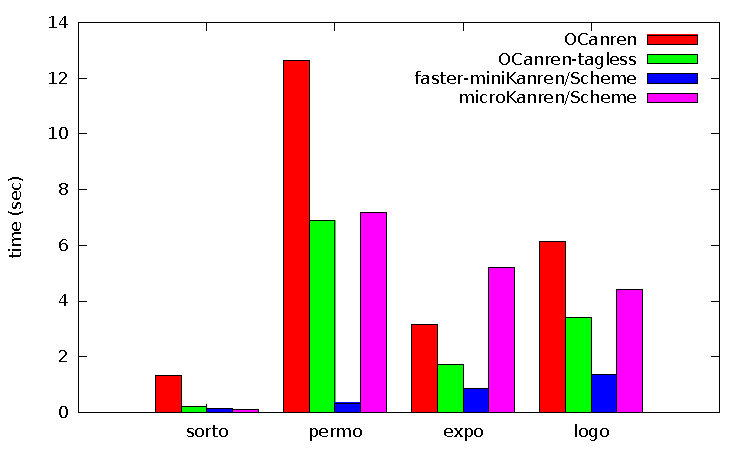
\includegraphics{graph1.pdf}
\caption{The First Set of Benchmarks}
\label{eval:first}
\end{figure}

\begin{figure}[h]
\centering
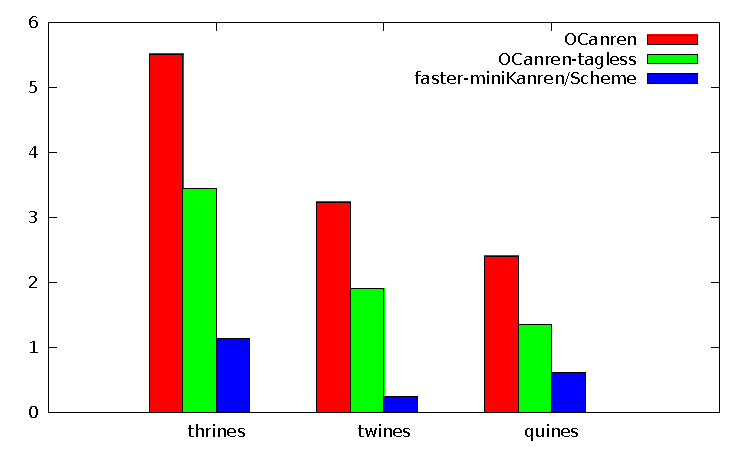
\includegraphics{graph2.pdf}
\caption{The Second Set of Benchmarks}
\label{eval:second}
\end{figure}

\section{Limitations and Future Work}

\label{sec:limitations}

In this section we discuss the limitations 
of constructive negation in general 
and our implementation in particular. 
Also we consider possible directions for future work.

\subsection{Type Constraints}

Although the program written in \textsc{OCanren} typechecks statically 
(thus, for example, preventing the user from unifying two terms of distinct types),
at runtime the type information is erased.
In the presence of even regular disequality constraints
it can lead to the incorrect results.
As an example, consider the following program:

\begin{minipage}[h]{\textwidth}
\begin{lstlisting}[
  % caption={An example of unsoundness in the presence of types},
  label={lst:types-unsound}
]
type bool = true | false

let g = 
  fresh (x y z : bool) (
    (x =/= y)
    (y =/= z)
    (z =/= x)
  )
\end{lstlisting}
\end{minipage}

The goal \lstinline{g} states that there
exists at least three different non-equal 
terms of type \lstinline{bool},
which, as we know, is not true.
Yet the query \lstinline{run g} will succeed.

In order to prevent unsoundness in cases like this,
type information in the form of \emph{type constraints}
should be somehow attached to the variables at runtime.
The satisfiability of type constraints then should 
be rechecked each time when the new disequality is added to some variable.
An extension of \textsc{OCanren} with type constraints
is a direction for future work.

\subsection{Non-stratified Programs}

As we have already discussed in the section~\ref{sec:strat}
our current implementation handles only stratified logic programs.
One of the possible extensions is to support 
non-stratified programs, such as one given in Listing~\ref{lst:game},
with respect to well-founded and/or stable model semantics 
(see section~\ref{sec:related-works} for the details).

\subsection{Negation of Goals With an Infinite Number of Answers}

Consider the following program:

\begin{minipage}[h]{\textwidth}
\begin{lstlisting}[
  % caption={Relation defining a list of zeros},
  label={lst:zeros}
]
let zeros l =
  l === [0] 
  \/
  fresh (l') (
    (l === 0 :: l')
    (zeros l')
  )
\end{lstlisting}
\end{minipage}

The unary relation \lstinline{zeros} defines lists consisting of zeros.
Now, intuitively, the query \lstinline{run ~(zeros q)} should enumerate
all lists that are not built out of zeros only.
Yet this query will fail to deliver even a single answer.
Why? Consider its operational behavior.
First the positive version of the goal, that is \lstinline{zeros q}, should be executed.
Then all answers to this goal should be collected and complemented.
However, there is an infinite number of answers to \lstinline{zeros q}
and thus this process will never terminate. 

It is a significant drawback of constructive negation
that the negation of the goal cannot be computed
if the goal has an infinite number of answers.
This limitation cannot be avoided in general,
however in some cases it is possible to narrow 
the number of answers to some subgoal 
by the reordering of surrounding subgoals.
For example, the query \lstinline{run ~(zeros q) /\ (q === [1])}
can be executed in finite time by the reordering of conjuncts.
It seems that the best strategy is to delay 
negative subgoals as long as possible,
but we do not have a formal proof of that.

\section{Related Works}
\label{sec:relworks}

There is a predictable glitch in implementing \miniKanren for a strongly typed language.
Designed in the metaprogramming-friendly and dynamically typed realm of Scheme/Racket, the original
\miniKanren implementation pays very little attention to what has a significant importance in (specifically)
ML or Haskell. In particular, one of the capstone constructs of \miniKanren~--- unification~--- has to work for
different data structures, which may have types different beyond parametricity.

There are a few ways to overcome this problem. The first one is simply to follow the untyped paradigm and
provide unification for some concrete type, rich enough to represent any reasonable data structures.
Some Haskell \miniKanren libraries\footnote{\url{https://github.com/JaimieMurdock/HK}, \url{https://github.com/rntz/ukanren}}
as well as the previous OCaml implementation\footnote{\url{https://github.com/lightyang/minikanren-ocaml}} take this approach.
As a result, the original implementation can be retold with all its elegance; the relational specifications, however,
become weakly typed. The similar approach was taken in early works on embedding Prolog into Haskell~\cite{PrologInHaskell}.

Another approach is to utilize the \emph{ad hoc} polymorphism and provide a type-specific unification for each ``interesting'' type.
Some \miniKanren implementations, such as Molog\footnote{\url{https://github.com/acfoltzer/Molog}} and
MiniKanrenT\footnote{\url{https://github.com/jvranish/MiniKanrenT}}, both for Haskell, can be mentioned as examples.
While preserving strong typing, this approach requires a lot of ``boilerplate''
code to be written, so some automation, for example, using Template Haskell\footnote{\url{https://wiki.haskell.org/Template_Haskell}},
is desirable. In~\cite{TypedLogicalVariables} a separate type class was introduced to both perform the unification
and detect free logical variables in an end-user data structures. The requirement for an end user to provide a way to represent
logical variables in custom data structures looks a bit obtrusive for us since these logical variables would require a proper
handling in the rest of the code outside the logical programming subsystem.

There is, actually, another potential approach, but we do not know if anybody has tried
it: to implement unification for a generic representation of types as sum-of-products and fixpoints of
functors~\cite{InstantGenerics, ALaCarte}. Thus, unification would work for any types for which a representation
is provided. We assume that implementing this representation would require less boilerplate code to be written.

As follows from this exposition, a typed embedding of \miniKanren in OCaml can be done with
a combination of datatype-generic programming~\cite{DGP} and \emph{ad hoc} polymorphism. There are a
number of generic frameworks for OCaml (for example,~\cite{Deriving}). On the other hand, the support
for \emph{ad hoc} polymorphism in OCaml is weak; there is nothing comparable in power to Haskell
type classes, and even though sometimes the object-oriented layer of the language can be used to mimic
desirable behavior, the result, as a rule, is far from satisfactory. Existing proposals (for example,
modular implicits~\cite{Implicits}) require patching the compiler, which we tend to avoid.
The approach we take here is to use a purely \emph{ad hoc} approach for implementing the unification, since the features
which would provide a less \emph{ad hoc} solution are not yet well integrated into the language. To deal
with user-defined types in the relational subsystem, we propose to use their logical representations, which free an end user
from the burden to maintain logical variables, and we use generic programming to build conversions from and to logical
representations almost effortlessly.




\section{Conclusion}

We presented a strongly-typed implementation of \miniKanren for OCaml. Our implementation
passes all tests written for \miniKanren (including those for disequality constraints);
in addition we implemented many interesting relational programs known from
the literature. We claim that our implementation can be used both as a convenient
relational DSL for OCaml and an experimental framework for future research in the area of
relational programming.

%We also want to express our gratitude to William Byrd, who infected us with relational programming,
%and for the extra time he sacrificed as both our tutor and friend.


%% Acknowledgments
\begin{acks}                            %% acks environment is optional
                                        %% contents suppressed with 'anonymous'
  %% Commands \grantsponsor{<sponsorID>}{<name>}{<url>} and
  %% \grantnum[<url>]{<sponsorID>}{<number>} should be used to
  %% acknowledge financial support and will be used by metadata
  %% extraction tools.

  % This material is based upon work supported by the
  % \grantsponsor{GS100000001}{National Science
  %   Foundation}{http://dx.doi.org/10.13039/100000001} under Grant
  % No.~\grantnum{GS100000001}{nnnnnnn} and Grant
  % No.~\grantnum{GS100000001}{mmmmmmm}.  Any opinions, findings, and
  % conclusions or recommendations expressed in this material are those
  % of the author and do not necessarily reflect the views of the
  % National Science Foundation.


  We want to thank Dmitry Boulytchev and Ekaterina Verbitskaia
  for valuable comments on a draft version of the paper.
  This work was partially supported by 
  the grant \grantnum{GS100000001}{18-01-00380}
  from the \grantsponsor{GS100000001}{Russian Foundation for Basic Research}{https://www.rfbr.ru/rffi/eng}
  and the grant from JetBrains Research.

\end{acks}

%% Appendix
% \appendix
% \section{Appendix}

% The default list of authors is too long for headers}
% \renewcommand{\shortauthors}{G. Zhou et al.}

%\setmonofont[Mapping=tex-text]{CMU Typewriter Text}
\bibliography{main}

\end{document}
